\chapter{Resultados}

\section{Separação de padrões}


Alguns resultados iniciais a partir do protocolo descrito na Seção~\ref{sec:separacao_padroes} já foram obtidos e serão discutidos
nesta seção.

A Figura~\ref{fig:avg_activity} apresenta a ativação média das populações de GCs para o modelo de controle (sem neurogênese) e
para os modelos com neurogênese em diferentes níveis de conectividade das iGCs com o CE. No modelo de controle, onde todas as GCs
são maduras, a ativação média da população, definida pela porcentagem de células que dispararam ao menos uma vez durante o
intervalo de \SI{1000}{\milli\second} da simulação, foi de 12.46\%, um nível de ativação esparsa, mas não tão baixo quanto o
observado no DG. Em simulações futuras, será analisado o impacto de um aumento de sinapses inibitórias no circuito.

A introdução de iGCs no circuito altera significativamente essa dinâmica. Conforme a conectividade das iGCs aumenta, a sua taxa de
ativação cresce acentuadamente, o que é consistente com sua maior excitabilidade intrínseca. No cenário de 100\% de conectividade,
praticamente toda a população de iGCs se torna ativa em resposta a um padrão de entrada. Esse aumento na atividade das iGCs eleva
a ativação geral da população de GCs.

Em contrapartida, observa-se uma diminuição progressiva na atividade das GCs maduras (mGCs) à medida que a conectividade das iGCs
aumenta. Este resultado sugere a existência de um mecanismo de competição inibitória, onde as iGCs, ao serem fortemente ativadas,
acabam por suprimir indiretamente a atividade das mGCs através dos interneurônios compartilhados.

Contudo, a supressão observada nas mGCs não é tão acentuada quanto a reportada em outros modelos~\cite{kimEffect2024}, o que pode
indicar novamente que a força da inibição no modelo atual seja insuficiente. Uma hipótese para essa discrepância é a ausência de
uma via inibitória direta das iGCs para as mGCs, um mecanismo descrito por~\citeonline{lunaAdultborn2019} que não foi
implementado. A inclusão dessa conexão direta é uma via promissora para futuras investigações, podendo conferir maior realismo
biológico ao modelo e também será explorada no projeto.

\begin{figure}[H]
    \centering
    \caption{Ativação média da população (\%) por modelo. O eixo vertical possui uma descontinuidade e duas escalas diferentes para melhor visualização. O erro é representado pela área sombreada.}
    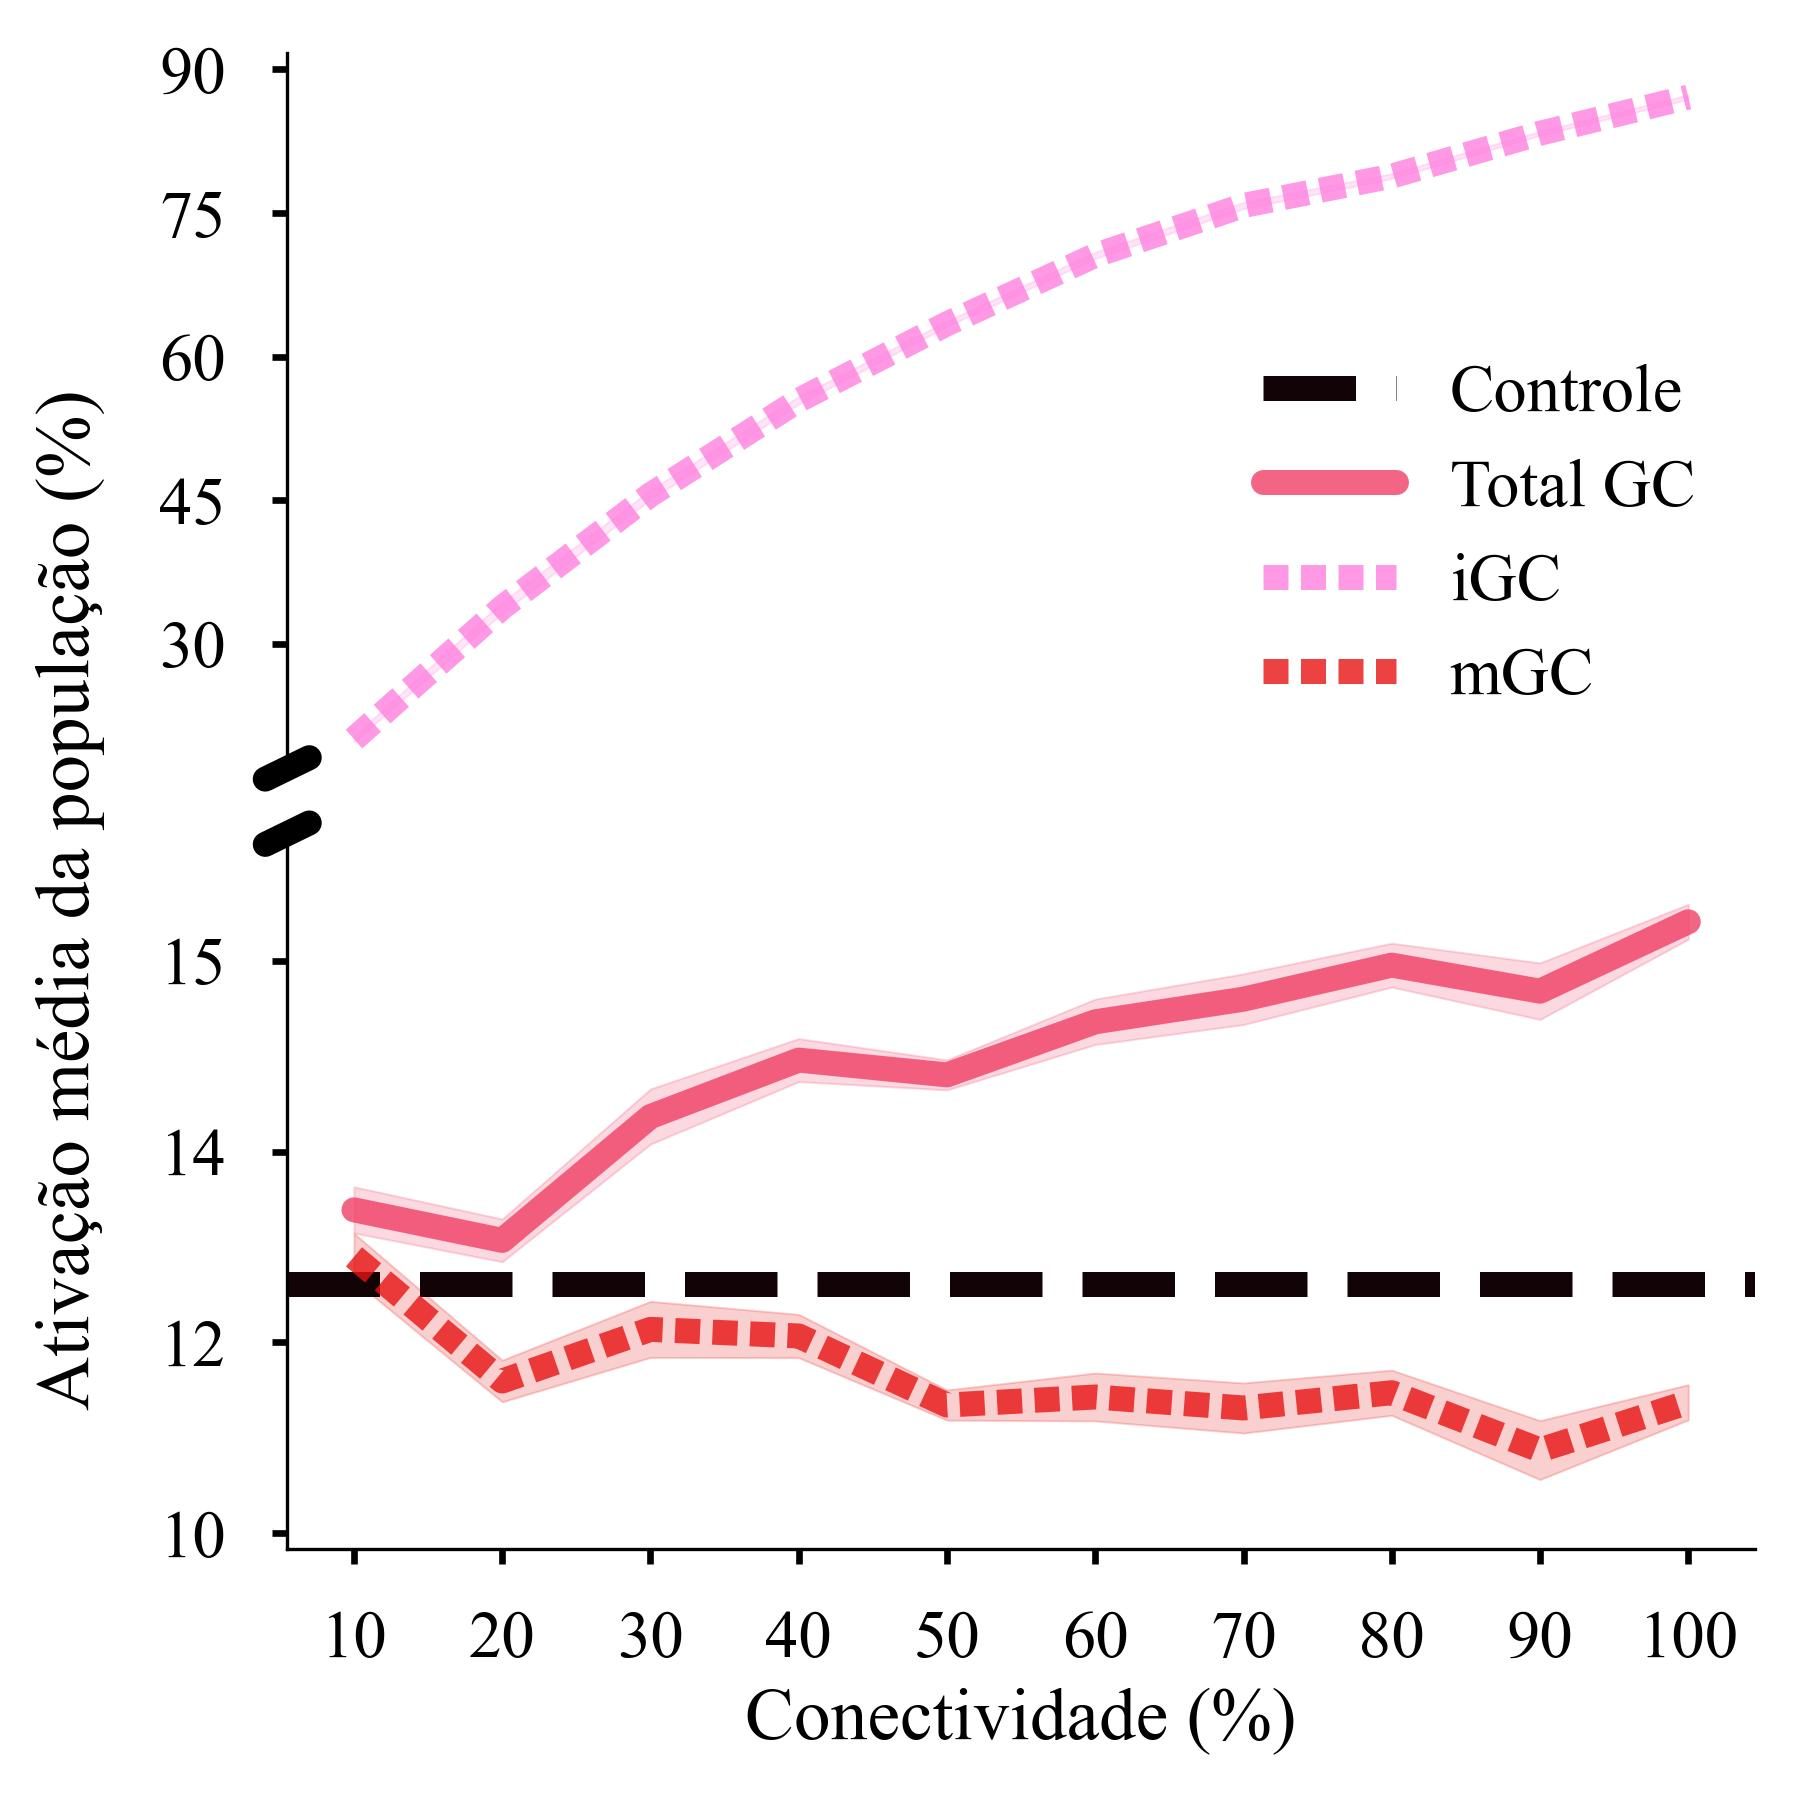
\includegraphics[width=0.7\textwidth]{figuras/plots/avg_activity}
    \label{fig:avg_activity}
\end{figure}


A Figura~\ref{fig:pattern_separation} aprofunda a análise ao detalhar o grau de separação de padrões ($\mathcal{S}_D$) em função
da similaridade dos padrões de entrada. Um valor de $\mathcal{S}_D > 1$ significa que a representação de saída no DG é mais
distinta do que a representação de entrada no CE. De forma geral, observa-se que todos os modelos, incluindo o de controle,
alcançam uma separação de padrões mais elevada para entradas altamente similares. Isso ocorre porque, matematicamente, pequenas
diferenças na codificação de saída são amplificadas quando a sobreposição na entrada é muito grande. O desempenho do modelo de
controle com entradas de baixa similaridade foi subótimo, não conseguindo separar os padrões de forma eficaz, o que pode ser
novamente atribuído à esparsidade insuficiente da rede, como discutido anteriormente. A introdução da neurogênese exacerba essa
limitação: à medida que a conectividade das iGCs aumenta, a capacidade de separação de padrões da rede diminui progressivamente. O
modelo com 100\% de conectividade das iGCs apresenta o pior desempenho em todas as condições de similaridade. O mecanismo
subjacente a essa deterioração é a ativação promíscua das iGCs, que, devido à sua alta excitabilidade, tendem a formar um mesmo
subconjunto de neurônios ativos em resposta a padrões de entrada distintos, reduzindo a dissimilaridade das representações na
saída e, consequentemente, o grau de separação de padrões.

\begin{figure}
    \centering
    \caption{Grau de separação de padrões ($\mathcal{S}_D$) por modelo e nível de similaridade de entrada. A linha tracejada
    representa um grau de separação de 1, valores acima disso indicam que houve separação de padrões, enquanto que valores abaixo
    disso indicam que não houve separação. O erro é representado pela área sombreada.}
    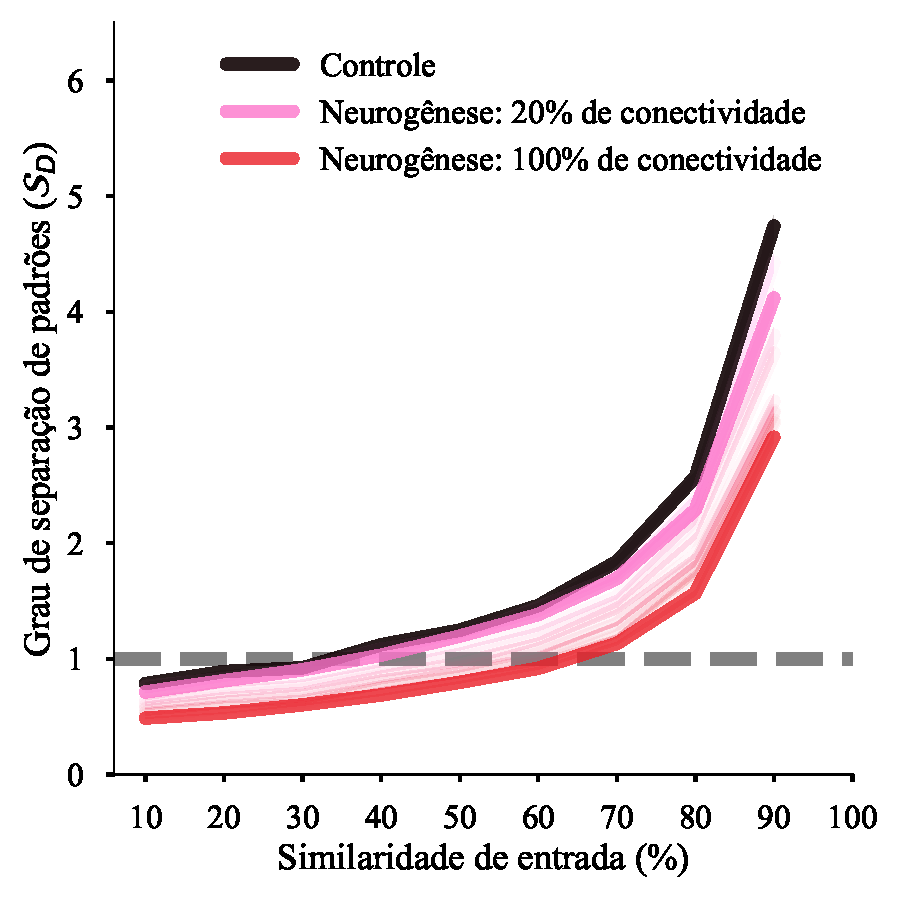
\includegraphics[width=0.7\textwidth]{figuras/plots/pattern_separation}
    \label{fig:pattern_separation}
\end{figure}

Para dissecar as contribuições individuais de cada população neuronal, a Figura~\ref{fig:avg_pattern_separation} apresenta o
$\mathcal{S}_D$ médio, agregado sobre todos os níveis de similaridade. Esta análise confirma a tendência observada anteriormente,
mostrando que a capacidade de separação de padrões do conjunto total de GCs diminui com o aumento da conectividade das iGCs. A
análise das subpopulações revela uma clara dicotomia funcional: as iGCs, isoladamente, nunca alcançam um $\mathcal{S}_D > 1$,
indicando que, em vez de separar, elas integram os padrões de entrada, tornando-os mais similares. Em contraste, as mGCs
demonstram uma robusta capacidade de separação de padrões em todos os modelos. 

O desempenho das mGCs melhora ligeiramente com o aumento da conectividade e atividade das iGCs, provavelmente um subproduto do
aumento da inibição global na rede, que, embora insuficiente, pode estar tornando a atividade das mGCs marginalmente mais esparsa.
Um modelo de regressão linear simples foi utilizado para avaliar a relação entre o nível de conectividade das iGCs e o grau de
separação de padrões das mGCs. O modelo encontrou uma relação significativa, embora fraca, entre o nível de conectividade e o grau
de separação de padrões ($F(1, 8) = 7.83, p = 0.023, R^2 = 0.49, \mathcal{S}^{mGC}_D = 1.76 + 0.13 \times \text{Conectividade}$).

Esses achados corroboram a teoria proposta por~\citeonline{kimEffect2024}, que sugere um papel das mGCs como separadoras de
padrões e das iGCs como integradoras. Resta investigar, em experimentos futuros, qual o impacto dessa codificação mista e do
fortalecimento da separação nas mGCs para as funções de memória no CA3.

\begin{figure}
    \centering
    \caption{Grau de separação de padrões ($\mathcal{S}_D$) médio por modelo e população. A linha tracejada em preto representa o
    $\mathcal{S}_D$ do controle, enquanto que a em cinza representa um grau de separação de 1. O erro é representado pela área
    sombreada; neste caso, o erro é muito grande, visto que o $\mathcal{S}_D$ varia muito entre diferentes níveis de similaridade
    na Figura~\ref{fig:pattern_separation}.}
    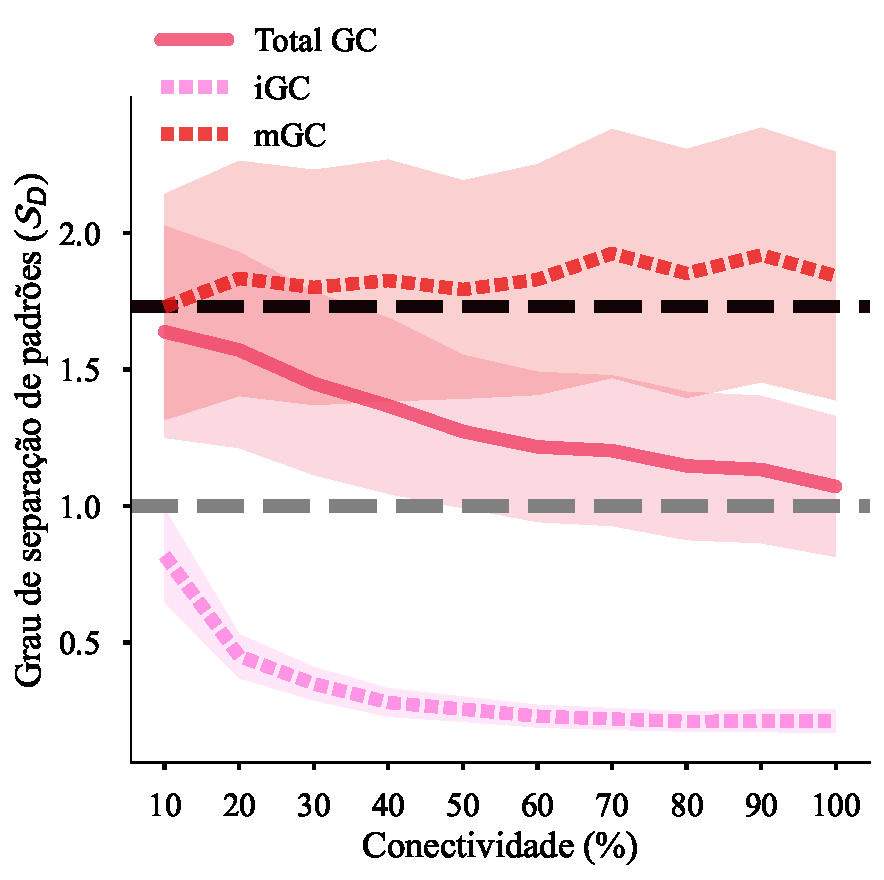
\includegraphics[width=0.7\textwidth]{figuras/plots/avg_pattern_separation}
    \label{fig:avg_pattern_separation}
\end{figure}


\section{Resultados esperados}

Espera-se que a presença de iGCs prejudique o completamento de padrões no CA3, devido a uma maior ativação de assembleias
neuronais não relacionadas ao padrão de entrada, um efeito consistente com resultados experimentais que sugerem uma ativação
promíscua de assembleias por parte das iGCs devido à sua alta excitabilidade~\cite{koSystems2025}. Adicionalmente, na simulação da
maturação temporal, espera-se que as iGCs passem a codificar os padrões no tempo, integrando informações que foram apresentadas
enquanto eram jovens, corroborando seu papel como integradoras temporais, como proposto por~\cite{aimoneComputational2009}.
Teoriza-se, portanto, que as mGCs teriam um papel predominante na separação de padrões específicos e distintos, enquanto as iGCs,
ao longo de sua maturação, se especializariam na separação de padrões próximos no tempo, ou seja, aqueles que codificaram durante
sua fase imatura.
